\begin{figure}[t]
\noteBox{Protocol}{
A protocol in computing and telecommunications is a set of rules and conventions that govern the exchange of data between devices. It defines the procedures for data transmission, including how data is formatted, transmitted, and received. Protocols ensure that devices can communicate effectively and understand each other, regardless of differences in their underlying hardware or software.
}
\end{figure}

\section{Entity Authentication}
\label{sec::chp2::authentication}

Entity authentication or \textit{identification} is the process of verifying the identity of a user, device, or system before granting access to sensitive information or functionality. It allows the \textit{claimant} to reassure another entity (the \textit{verifier}) of their identity. In related literature~\cite{menezes_handbook_1997}, the terms identification and entity authentication are often used interchangeably. Identification protocols are ubiquitous; we encounter them most commonly when logging into web applications. They are also used when unlocking a car with a wireless key fob or accessing an ATM.

\textbf{Password-based authentication} is the most prevalent form of entity authentication, tracing its history back to the early days of computing. This form of authentication is considered weak due to the vulnerabilities associated with user-chosen passwords. The password itself is a string—often a minimum of six characters—selected and memorised by the user, serving as a shared secret between the user and the system (verifier). The password string is linked to a claim of identity, such as a unique username or email address. We explore password-related topics in depth in Section~\ref{sec::chp2::password}.

\textbf{Personal identification numbers (PINs)} are commonly used on mobile devices or in conjunction with banking cards to prevent unauthorised access to personal devices or other physical possessions. PINs are typically four or six digits long and are most commonly employed as a secondary form of authentication.

Fixed secret schemes, such as passwords and PINs, are susceptible to replay attacks due to eavesdropping. \textbf{One-time passwords (OTPs)} mitigate this risk by ensuring that each password is used only once per login attempt. There are two variants of OTP: (1) Hash-based OTP (HOTP) and (2) Time-based OTP (TOTP). HOTP relies on a counter that increments with each use, whereas TOTP is based on the current time, typically changing every 30 seconds. As a result, TOTP is short-lived and requires only reasonably synchronised clocks, whereas HOTP necessitates synchronisation between both the client and the server. Due to its simplicity and security benefits, TOTP is the more commonly used algorithm.

Protocols that require interaction between entity $A$ (the \textit{claimant}, who is proving their identity) and entity $B$ (the \textit{verifier}) are known as \textbf{challenge-response authentication}. These protocols utilise a time-variant challenge to defend against active attacks; the challenge is provided by entity $B$ (the verifier—a system or device). Kerberos and Needham–Schroeder are examples of symmetric-key, challenge-response-based protocols. We discuss zero-knowledge-based schemes in Section~\ref{sec::chp2::identity-based-ciphers} and utilise them in Chapter~\ref{chp::deeid}.


\section{Attacks on Entity Authentication Protocols}
\label{sec::chp2::attacks-on-auth}

There are various security threats to identification protocols~\cite{menezes_handbook_1997}:  

\begin{itemize}
\item
  \emph{Impersonation}. Pretending to be a different person.
\item
  \emph{Replay attack}. Use of information from a previously used
  protocol process, e.g.~re-use of a poor signature.
\item
  \emph{Interleaving attack}. Multiple concurrent execution of the
  protocol and using selective information for possible attacks.
\item
  \emph{Reflection Attack}. Attack on a challenge-response method to
  essentially tricking the challenger into providing itself with the
  answer.
\item
  \emph{Forced Delay}. Requires intercepting a message and delaying it
  until some later time (thus not a replay attack).
\item
  \emph{Chosen-text Attack}. Strategically choosing challenges in an
  attempt to extract information about the prover's secret information.
\end{itemize}


\section{Multi-Factor Authentication}
\label{chp2::multi-factor-authentication}

\begin{figure}
    \centering
    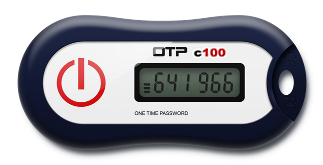
\includegraphics[width=0.33\linewidth]{figs/otp_hardware.jpg}
    \caption{Photograph of a hardware-based OTP device that is capable of generating event-based and time-based one-time passwords. This form is a visual-based hardware OTP as it requires the user to identify the digits and enter them onto another device.}
    \label{fig:otp-hardware}
\end{figure}

Multi-factor authentication (MFA) is a layered approach to security and access control, combining multiple authentication methods to enhance the overall security of a system. Applications typically implement two-factor authentication (2FA), which pairs password-based authentication with an OTP or SMS verification. In practice, OTP methods are commonly implemented through mobile phone applications.

The distinction between what constitutes multi-factor authentication is not always clear-cut. Often, if the \textit{user} is required to interact with multiple systems, it is considered multi-factor authentication. However, when metadata---such as location and IP address---is used, it is less clear whether this qualifies as multi-factor authentication.

Use of multi-factor authentication comes often at a cost to usability. Users are often required to use a secondary device or have access to a mobile phone with LTE access. Use of multi-factor authentication provides additional costs to organisations too--an example of this is when Twitter forced non-paying users to switch from SMS-based 2FA to other forms of 2FA \cite{taylor_twitter_2023}. The reasoning for this was both cost (to Twitter) and the fact that SMS-based 2FA can be vulnerable for most users. The user experience of MFA has hardly changed over the last decade \cite{cristofaro_comparative_2014}, indicating a lack of research or adoption in the research.

The use of multi-factor authentication often comes at the cost of usability. Users are frequently required to utilise a secondary device or have access to a mobile phone with LTE connectivity. Additionally, multi-factor authentication imposes extra costs on organisations---an example of this is when Twitter required non-paying users to switch from SMS-based 2FA to alternative forms of 2FA~\cite{taylor_twitter_2023}. The rationale behind this decision was both the cost to Twitter and the vulnerability of SMS-based 2FA for most users. The user experience of MFA has remained largely unchanged over the past decade~\cite{cristofaro_comparative_2014}, suggesting a lack of research in this area.

SMS-based multi-factor authentication (MFA) involves sending a one-time password (OTP) to the authenticating user via SMS. A mobile phone number is registered to the user's account prior to this authentication stage. However, SMS-based MFA is susceptible to SIM-swapping attacks and SMS interception. Despite these vulnerabilities, SMS-based MFA remains widely adopted due to its convenience and its straightforward usability for users.

One-time passwords (OTPs) are unique authentication secrets generated using a shared secret and are used only once per authentication transaction. Their uniqueness and time-sensitive nature make them resistant to replay attacks. In practice, OTPs are generated through mobile phone applications, dedicated hardware devices, or out-of-band channels.

Hardware tokens are physical devices that generate OTPs. Unlike SMS or app-based OTPs, these tokens operate independently of the user's mobile device or computer—reducing the risk of side-channel attacks. Hardware tokens are also less susceptible to hacking or phishing attacks, as they do not rely on potentially vulnerable network connections. Figure~\ref{fig:otp-hardware} illustrates an example of a hardware-based OTP generator.

\section{FIDO2}
\label{sec::chp2::fido2}

\begin{figure}[t]
    \centering
    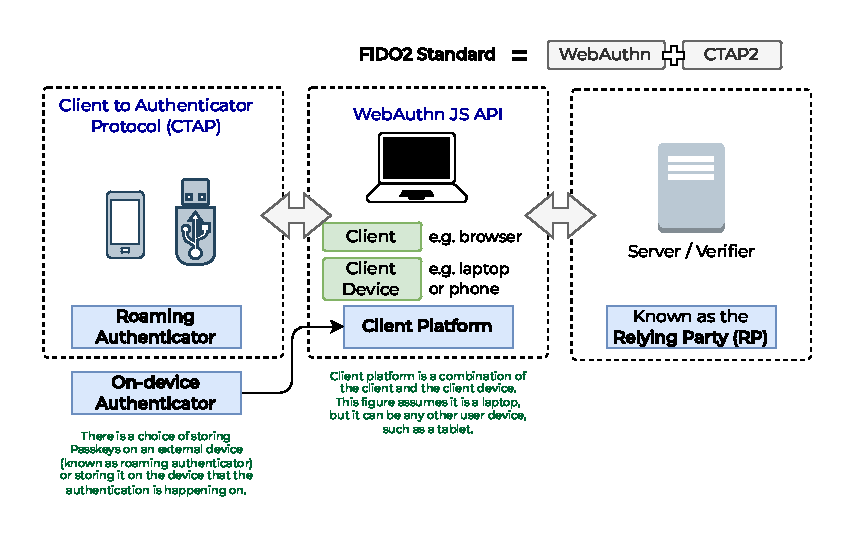
\includegraphics[scale=1.2]{figs/fido2_diagrams.pdf}
    \caption{Diagram showing the core components of the FIDO2 standard. FIDO2's primary intent is to replace password-based authentication with public-key cryptography-based authentication. It consists of the WebAuthn JS API and the protocol to communicate with external devices known as roaming authenticators. \srcOwnFig}
    \label{chp2::fig::fido2-diagram}
\end{figure}

FIDO2 is an authentication standard, which combines the WebAuthn~\cite{noauthor_web_2021} (Web Authentication API) and CTAP2~\cite{noauthor_client_2019} specifications. It represents the primary ongoing effort to replace password-based authentication (i.e., weak authentication) with strong authentication: public-key cryptography-based authentication. It consists of specifications for public-key cryptography-based authentication. Figure~\ref{chp2::fig::fido2-diagram} provides an illustration of the standard's core components.

The credentials in this ecosystem are known as WebAuthn credentials, FIDO credentials, or Passkeys. We will refer to them as Passkeys. Passkeys were introduced by Apple during WWDC 2022~\cite{noauthor_meet_2022} and have attracted considerable attention since then. The advantage of Passkeys for companies like Apple is that they can utilise the biometric features on the device to enhance the authentication experience for the user. However, a drawback is that users are locked into their platforms, as Passkeys are stored on iCloud, or they may lack the knowledge to transfer keys.

The Web Authentication API (WebAuthn)~\cite{noauthor_web_2021} is the specification and JavaScript API developed by W3C and the FIDO Alliance to enable public-key cryptography-based authentication. It is an extension of the Credential Management API. WebAuthn provides the necessary functions to interact with the verifier (server or relying party) and authenticators (which can be on-device or external—roaming authenticators). The Client to Authenticator Protocol (CTAP), currently in version 2 (CTAP2), is the specification that enables authenticators to interact with the WebAuthn API and the client.

FIDO2 is an initiative of the FIDO (Fast IDentity Online) Alliance, an open standard association formed through collaboration among various companies. The association was launched in February 2013 with the aim of creating and promoting a password-less authentication standard within the community. They define their mission as \textit{``authentication standards to help reduce the world's over-reliance on passwords.''} The executive leadership of the alliance includes members from Google, Amazon, Intel, Thales, Apple, Microsoft, and Docomo.

The work of the FIDO Alliance has been hindered by confusion and complexity, leading to a lack of widespread adoption. The maze of specifications, insufficient developer support, and evolving terminologies have made it challenging for developers to implement FIDO2 effectively. The alliance and its output exemplify a design-by-committee approach. Some literature~\cite{farke_you_2020, ghorbani_lyastani_is_2020} has examined the usability of FIDO2 systems in practice, concluding that users often revert to passwords or password managers due to their speed and convenience. Currently, FIDO2 is primarily used for second-factor authentication.

The journey of the FIDO Alliance began with the \texttt{Universal Authentication Framework (UAF)} and \texttt{Universal 2nd Factor (U2F)} standards in 2014. \texttt{Universal 2nd Factor (U2F)} is the standard used to enable two-factor authentication (2FA) through USB HID or NFC. It was succeeded by the Client to Authenticator Protocol 1 (\textbf{\texttt{CTAP1}}) standard, which provides a generalised interaction between the client device and secondary devices.


\section{Secure Hardware}
\label{sec::chp2::secure_hardware}

Isolated hardware with its own operating system can be used to protect user secrets, particularly on mobile phones and wearable devices. These devices store sensitive information such as passwords, financial data, and biometrics, and are ubiquitous; however, they also host numerous untrusted applications that may attempt to access this information. Most importantly, such devices can easily fall into the wrong hands. A response to these threats is dedicated hardware, or a segment of a System-on-Chip (SoC), separated from the rest of the system. This dedicated hardware is referred to as a Trusted Execution Environment (TEE) or a Secure Enclave.

A Trusted Execution Environment (TEE) is a dedicated area of the main processor with its own operating system (for example, on Android, the operating system running on the secure enclave is \fun{Trusty~TEE}~\cite{android_trusty_tee}). The purpose of such architectures is to isolate critical functions and protect cryptographic secrets in isolated contexts (enclaves) from the rest of the system. The remainder of the system is often referred to as the Rich Execution Environment (REE).

Most smartphone manufacturers now build secure enclaves directly into their devices' hardware. Apple design and manufacture their own SoCs and refer to the dedicated secure hardware as the \textit{Secure Enclave}. Other manufacturers, such as Samsung, use ARM-based processors and therefore adopt the \textit{ARM TrustZone} architecture. TEEs in mobile devices store passwords, PINs, biometric data, and other similar secrets. They protect user data by, for example, rate-limiting PIN attempts (with exponential delays) even when a malicious actor has physical access to the device. Biometric data can be stored and processed within the secure enclave; for instance, Touch ID, Face ID, and Optic ID on Apple devices~\cite{apple_biometric_security} are stored and processed exclusively within the secure enclave. On Android, developers can access the TEE via the \fun{Keystore}~API~\cite{android_keystore_api}. Despite the availability of this API, it has been shown~\cite{blessing2025keydroidlargescaleanalysissecure} that most Android applications do not use it for secret storage.

A Hardware Security Module (HSM) is dedicated hardware designed to manage cryptographic secrets. For example, in the cloud, an HSM may be used to avoid loading cryptographic keys into the memory of the main web server. Such isolation prevents leakage and unauthorised access to the keys by other applications.
